\chapter{Related work}
\section{Convoying}
Robotic convoying is a significant research problem in mobile robotics. This problem has been addressed from different points of view, e.g., artificial vision, control theory, artificial intelligence, etc. \cite{article:convoy_comm}. Most existing mobile robot systems still involve a single robot working alone, while there are a wide range of potential applications for robots acting in concert \cite{article:convoy_comm}.

The authors of \cite{article:guidance_control} discuss how a following robot imitates its lead robot, where each of the following robots track the angular and linear velocity of its lead robot. They also presented how to convoy with constant distance between robots while analyzing the case as Velocity Pursuit, Deviated Pursuit, and Proportional Navigation.

\section{Potential Fields}
The study of groups of multiple autonomous mobile robots has been of great interest \cite{article:motion_planning_apf}. In high-speed convoying, fast and efficient coordinated maneuvers are a must, as well as quickly processing data to make a decision. Biologists have observed remarkable group-level characteristics in animal aggregations such as swarms, flocks, school and herds \cite{article:motion_planning_apf}. Some of these characteristic are the ability to make very fast and efficient coordinated maneuvers, quickly process data and to cooperatively make decisions. Thus, there is a significant interest within the robotic community, to better understand the biological imperative and exploit it by incorporating similar principles in artificial robot collectives.  

Researchers typically refer to the use of potential field as a means for assisting a robot to move from one initial configuration to a desired final configuration without colliding with any obstacles. Potential fields consist of force vectors, caused by the obstacles or target positions, which may be linear or tangential and they may have characteristics of repulsive, attractive or random, depending on the state of the agent with respect to its environment \cite{article:apf}. It was originally developed as an on-line collision avoidance approach, applicable when the robot does not have a prior model of the obstacles, but rather senses them during motion execution \cite{article:real_time_avoidance_manip}. The most common potential field function is defined as:

\begin{equation} \label{eq:potential_fields}
F(q)=-\nabla(U_a(q)+U_r(q))
\end{equation}

It is defined over free space as the sum of an $U_a$ attractive potential pulling the robot toward the goal configuration and a $U_r$ repulsive potential pushing the robot away from the obstacles \cite{article:potential_fields_convoy}. This model attempts to find a collision-free, feasible, path in the neighborhood of the initial estimate. The goal is to define a path for the robot to follow, starting from the initial position moving towards the end/goal position calculated by the negative gradient of the entire field. If the start and the goal configurations cannot be connected through a sequence of feasible configurations, the initial path is then assumed not to lead to a solution. The potential field method has increased in popularity for the control of mobile robots, due to its mathematical simplicity \cite{article:potential_fields_convoy}.

\section{Car models}
In order to study the dynamics of a vehicle system, these are typically modeled as a quarter car, a half car, and a full car.

\subsection{Quarter car}
%% FIXME source [12]
To model a car, the typical approach is to break it down into smaller parts, and then recombine the parts at the end. To begin with, a quarter car model is created, showing only one wheel, constrained to one dimension (vertical displacement,) and the associated suspension \cite{article:convoy_comm,article:motion_planning_apf}. The quarter car model is shown in figure \ref{fig:quarter_car}. The car body is represented by the mass M and is connected to a suspension system consisting of a spring K and a damper B . The suspension is connected to the tire which is modeled as a mass M and a spring K connecting it to the road.

\begin{figure}[t]
	\centering
	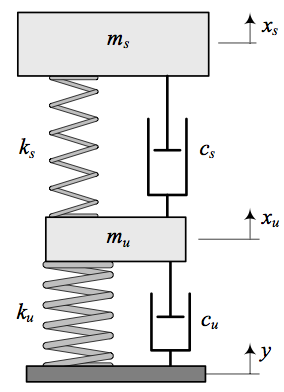
\includegraphics[width=0.25\textwidth]{figures/quarter_car.png}
	\caption{A generalized quarter car model with damped tires \cite{book:jazar}.}
	\label{fig:quarter_car}
\end{figure}

\subsection{Half car}
The half car model represents a two-dimensional view of the vehicle head-on as shown in figure \ref{fig:half_car}. Figure \ref{fig:half_car_pretty} shows the half car model overlaid on a car body as reference. It is actuated in two dimensions, vertical displacement and rotation about the center of gravity. Horizontal motion (slip) may also be shown on this model. As can be seen from the figure, the half car model is composed of two quarter car models acting on a common strut to realize roll.

\begin{figure}[t]
	\centering
	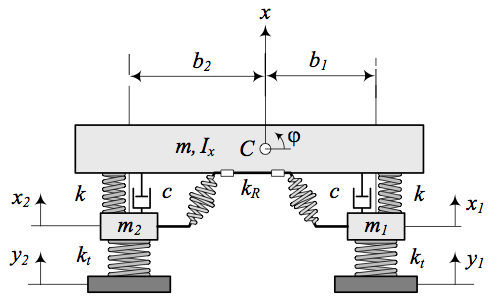
\includegraphics[width=0.7\textwidth]{figures/half_car.png}
	\caption{A generalized half car model with a roll-bar \cite{book:jazar}.}
	\label{fig:half_car}
\end{figure}

\begin{figure}[t]
	\centering
	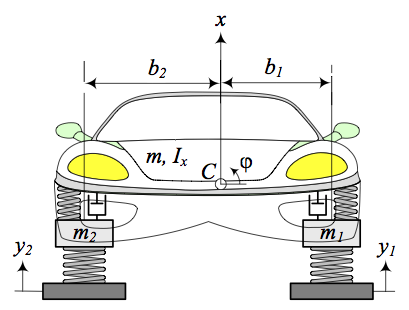
\includegraphics[width=0.7\textwidth]{figures/half_car_pretty.png}
	\caption{A generalized half car model overlaid on a car body \cite{book:jazar}.}
	\label{fig:half_car_pretty}
\end{figure}

\subsection{Full car}
Full Car. The full car model represents a three-dimensional view of the vehicle as shown in figure \ref{fig:full_car}. Figure \ref{fig:full_car_pretty} shows the full car model overlaid on a car body as reference. The full car model is composed of two half car models, one representing each side (front and back.) From these models one gets a combined roll and pitch. There is then a third (top down) view added to the model that allows for the calculation of yaw, and factors the input velocity into the model.

\begin{figure}[t]
	\centering
	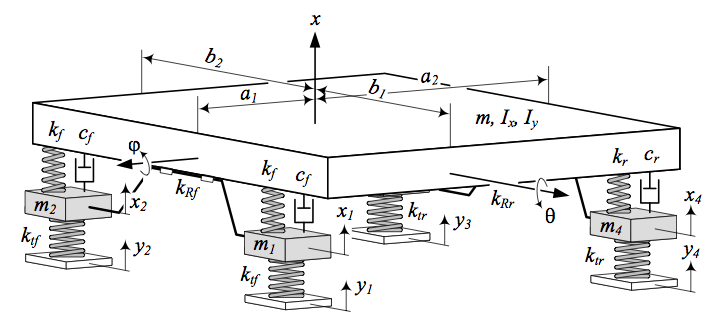
\includegraphics[width=0.9\textwidth]{figures/full_car.png}
	\caption{A generalized full car model with roll-bars \cite{book:jazar}.}
	\label{fig:full_car}
\end{figure}

\begin{figure}[t]
	\centering
	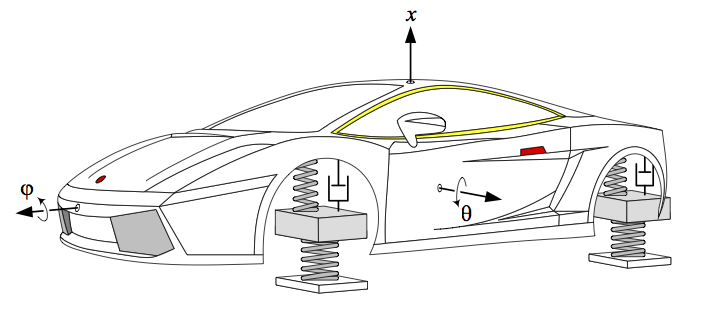
\includegraphics[width=0.9\textwidth]{figures/full_car_pretty.png}
	\caption{A generalized full car model overlaid on a car body \cite{book:jazar}.}
	\label{fig:full_car_pretty}
\end{figure}

